% Compiler: LaTeX => PDF

\documentclass[xcolor=dvipsnames]{beamer}

\mode<presentation>
{
	\usetheme{BerlinHUB}
	%\setbeamercovered{transparent}
}

\usepackage[ngerman]{babel}
\usepackage[utf8]{inputenc}

\usepackage{helvet}
\usepackage[T1]{fontenc}

%\usepackage{multimedia}
%\usepackage{graphicx}
%\usepackage[nolist]{acronym}

%\usepackage{stackengine}
%\usepackage{array}

%\usepackage{enumitem}
\usepackage{xcolor}


\def\frametitlesec{\frametitle{\arabic{section}.\hspace{0.5ex}\insertsection}}
\def\framesubtitles#1{\framesubtitle{\hspace{3.5ex}#1}}

%\setitemize{label=\usebeamerfont*{itemize item}%
%  \usebeamercolor[fg]{itemize item}
%  \usebeamertemplate{itemize item}}

\title[Streifenlichtprojektion]
{Streifenlichtprojektion und optische Analyse zur Oberflächeninspektion}

\author[D. Wagner, J. Spangenberg, L. Kramer]
{
	Dennis~Wagner
	\and
	Johannes~Spangenberg
	\and
	Leroy~Kramer
}

\institute[]
{
	Humboldt-Universität zu Berlin\\  
	Institut für Informatik\\
	Lehrstuhl Signalverarbeitung und Mustererkennung\\
	\vspace{1em}
	Semesterprojekt Signalverarbeitung\\
	bei Prof. Dr. Meffert
}

\date{17.04.2014}
\subject{Informatik}

% add logo of university
\pgfdeclareimage[height=0.75cm]{university-logo}{husiegel_bw_klein}
\logo{\pgfuseimage{university-logo}}

\setbeamercolor*{block title}{fg=white, bg=HUblue}


\begin{document}
\begin{frame}
	\frametitle{\mbox{}}
	\titlepage
\end{frame}

\begin{frame}
	\frametitle{Gliederung}
	\tableofcontents
\end{frame} 

% ---------------------------------------------------------------------------- %

\section{Motivation}
\begin{frame}
	\frametitlesec

	\textbf{Vermessungen komplexer Gebilde}
	\vfill
	\begin{columns}[T]
		\begin{column}{.4\linewidth}
			Qualitätskontrolle
			\begin{itemize}
				\item Carspector
			\end{itemize}
			\vspace{2em}
			Unterhaltung
			\begin{itemize}
				\item Kinect
				\item Modellerstellung
			\end{itemize}
		\end{column}
		\begin{column}{.4\linewidth}
			Dokumentation
			\begin{itemize}
				\item Artefakte
				\item Tatort
				\item Kartografie
				\item Reverse Engineering
			\end{itemize}
		\end{column}
	\end{columns}
	\vfill

\end{frame}


\begin{frame}
	\frametitlesec

	\textbf{Wie gelangt man an die Ausmaße eines Objektes?}
	\begin{itemize}
		\item Manuelle Vermessung
		\item Stereo-Vision
		\item Structure from Motion
		\item Time of Flight
		\item \dots
	\end{itemize}

\end{frame}


\begin{frame}
	\frametitlesec

	\vfill
	{\large\textbf{Unsere Methode: Streifenlichtprojektion}}
	\vfill
	\begin{itemize}
		\item Relativ günstig
		\item Messung ohne Kontakt zum Objekt
		\item Hohe Genauigkeit möglich
		\item Keine Epipolargeometrie
	\end{itemize}
	\vfill
	\begin{itemize}
		\item Langsam (im Vergleich zu \textit{Time of Flight})
		\item Abschattung des Lasers
	\end{itemize}
	\vfill

\end{frame}

% ---------------------------------------------------------------------------- %

\section{Umsetzung}
\begin{frame}
	\frametitlesec

	\begin{figure}
		\centering
		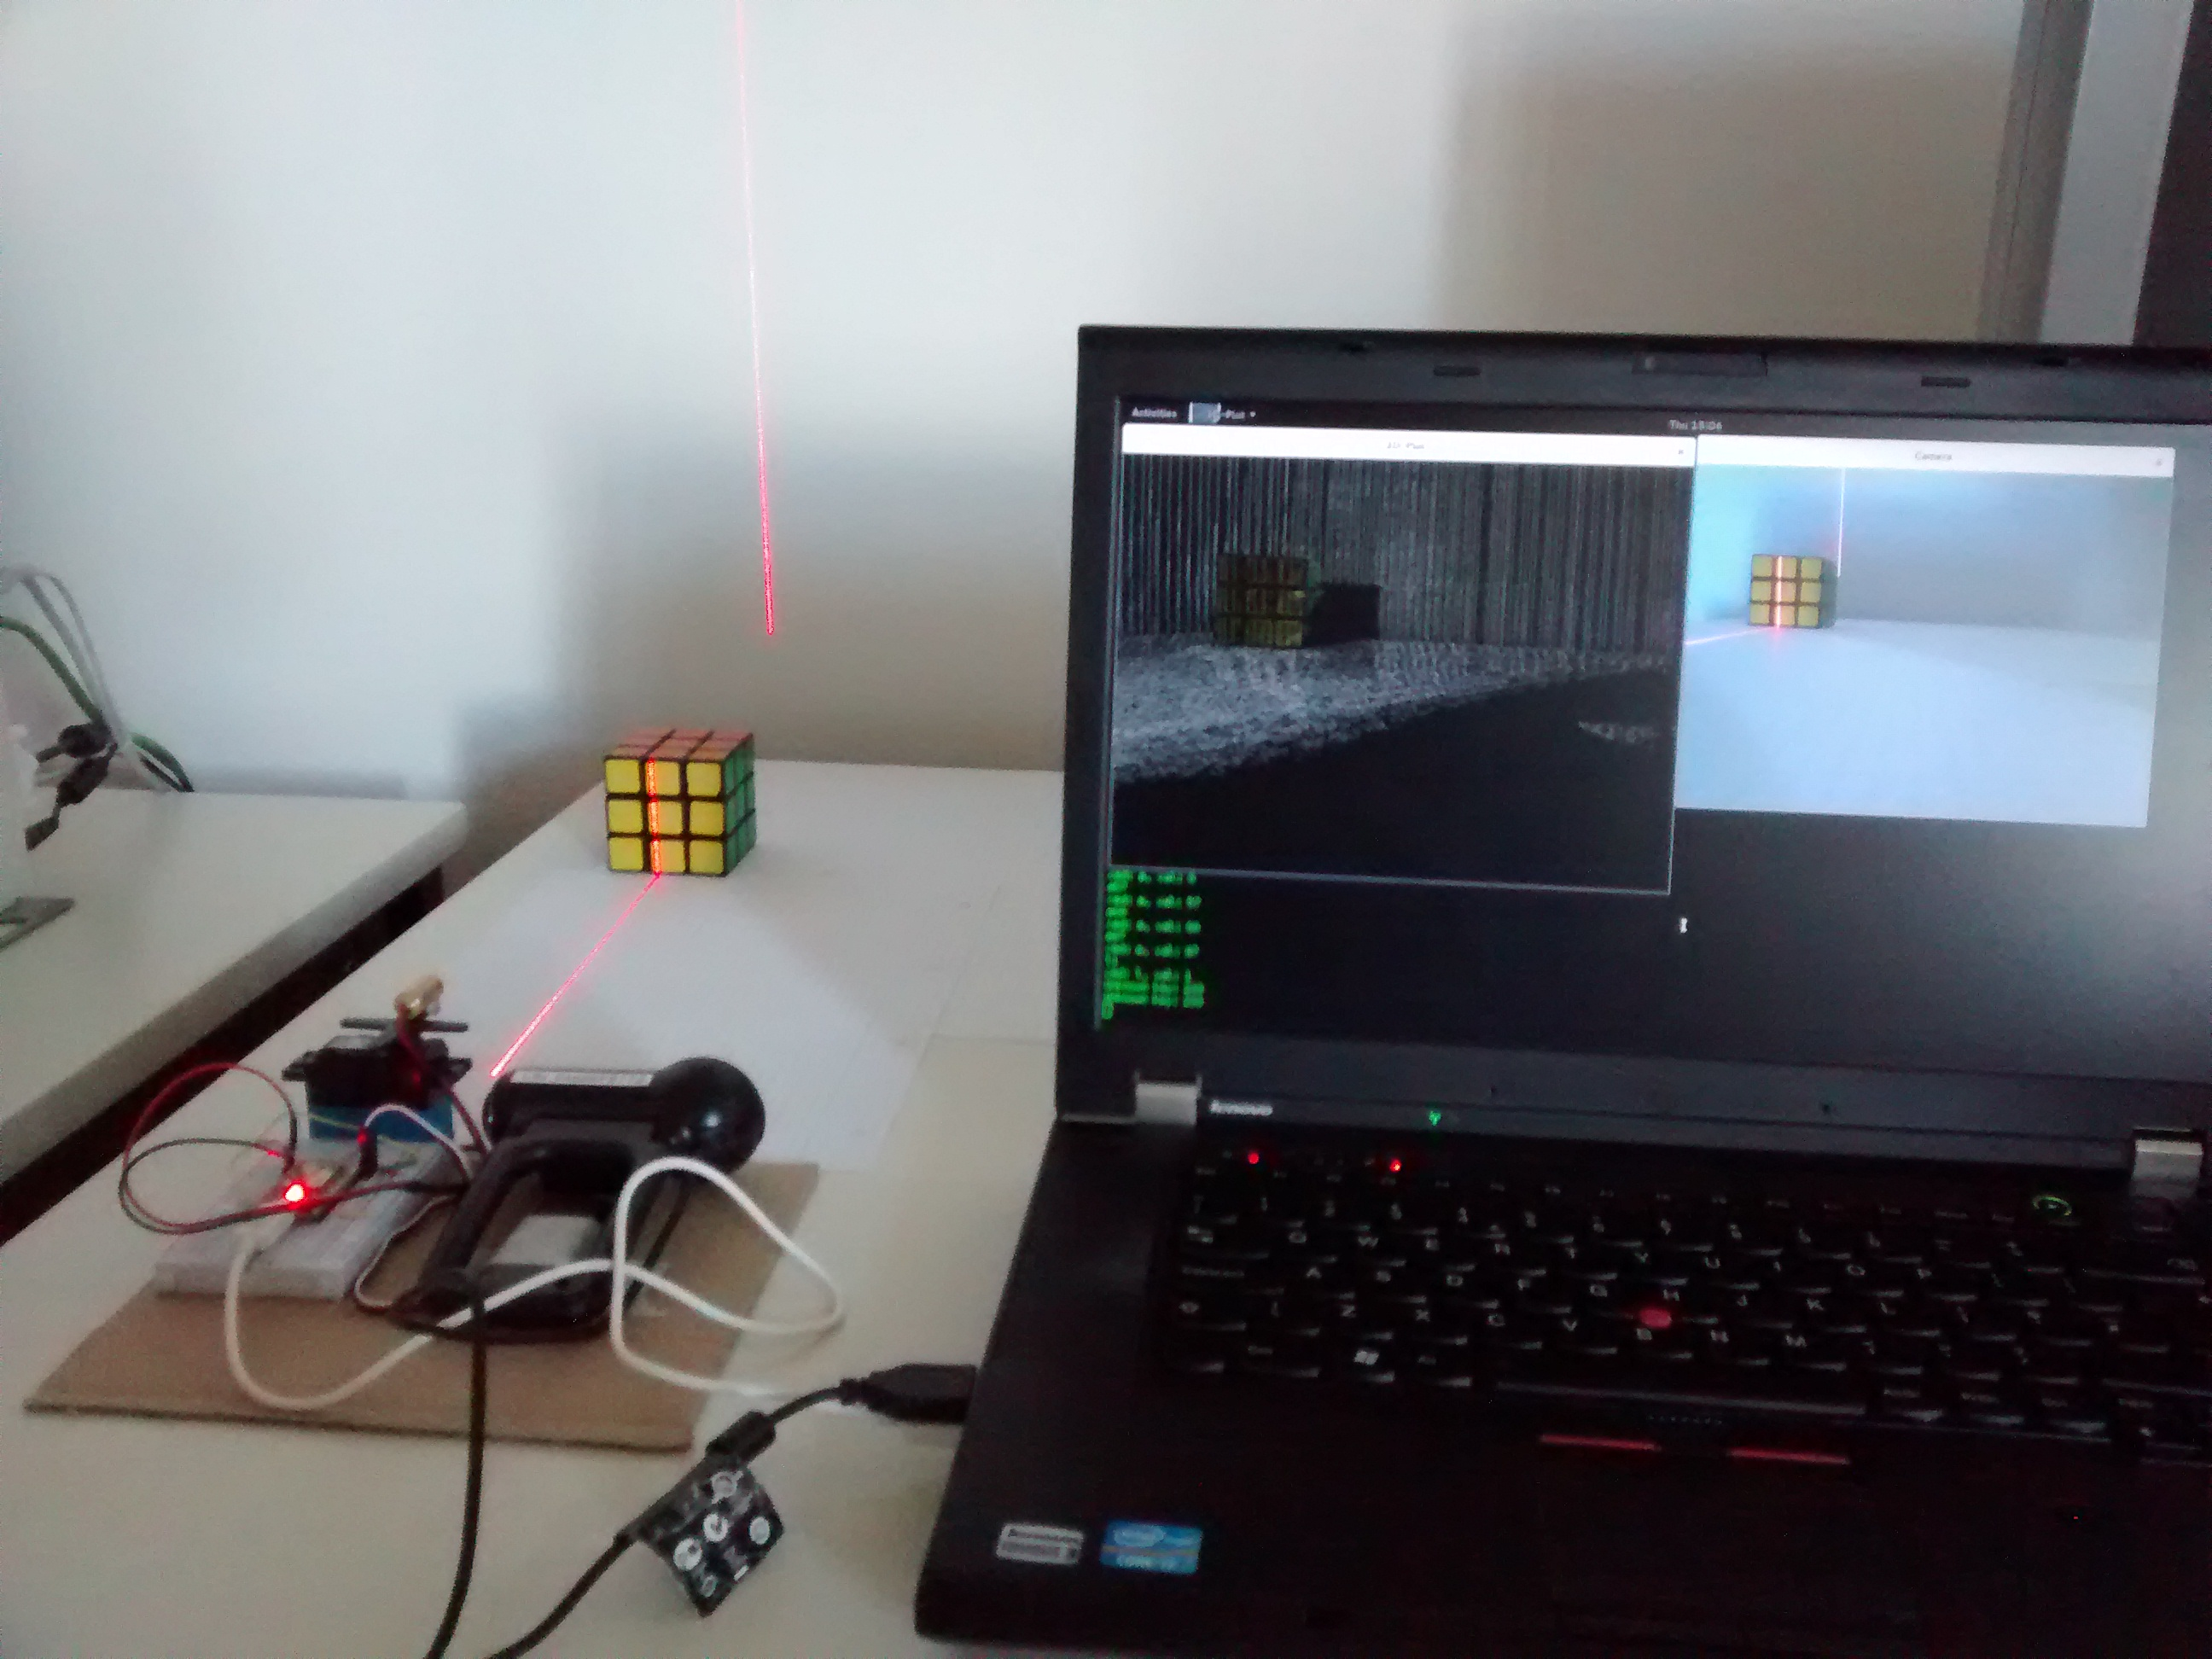
\includegraphics[width=0.8\linewidth]{includes/setup}
		\caption{Unser Setup im Betrieb}
		\label{fig:setup}
	\end{figure}

\end{frame}


%\subsection{Ablauf}
\begin{frame}
	\frametitlesec
	\framesubtitles{Ablauf}

	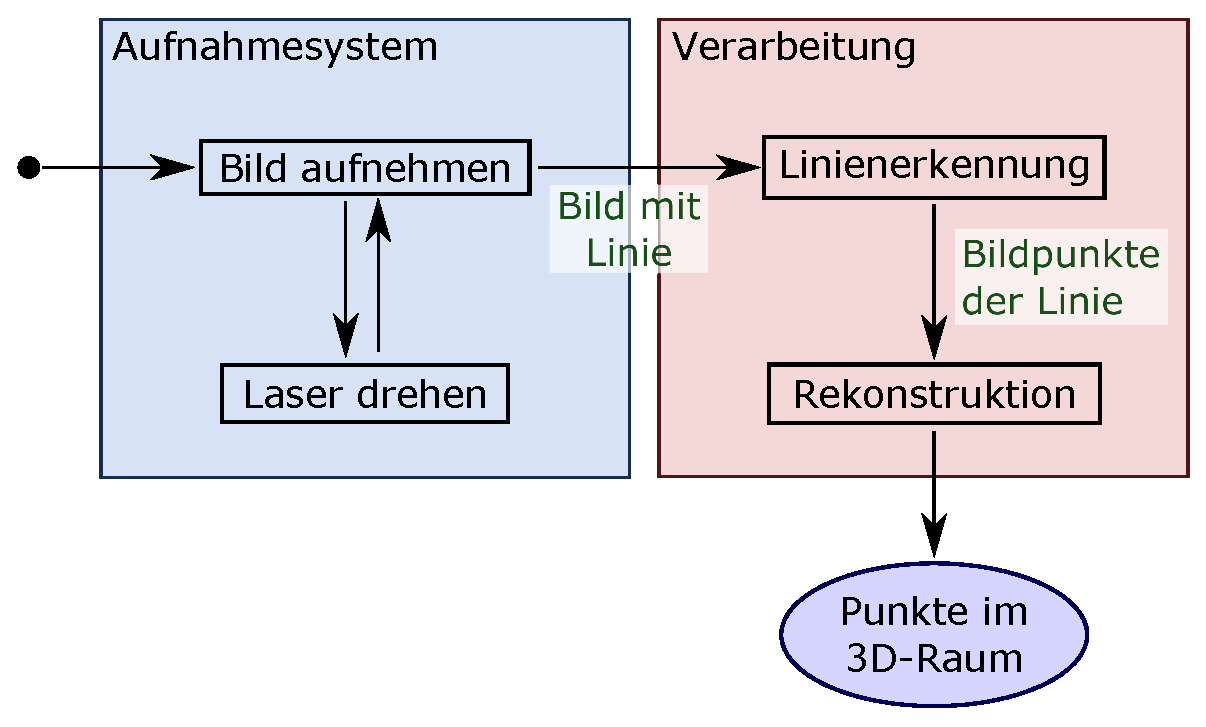
\includegraphics[width=\linewidth]{includes/blockbild}

\end{frame}


%\subsection{Hardware}
\begin{frame}
	\frametitlesec
	\framesubtitles{Hardware}

	\begin{figure}
		\centering
		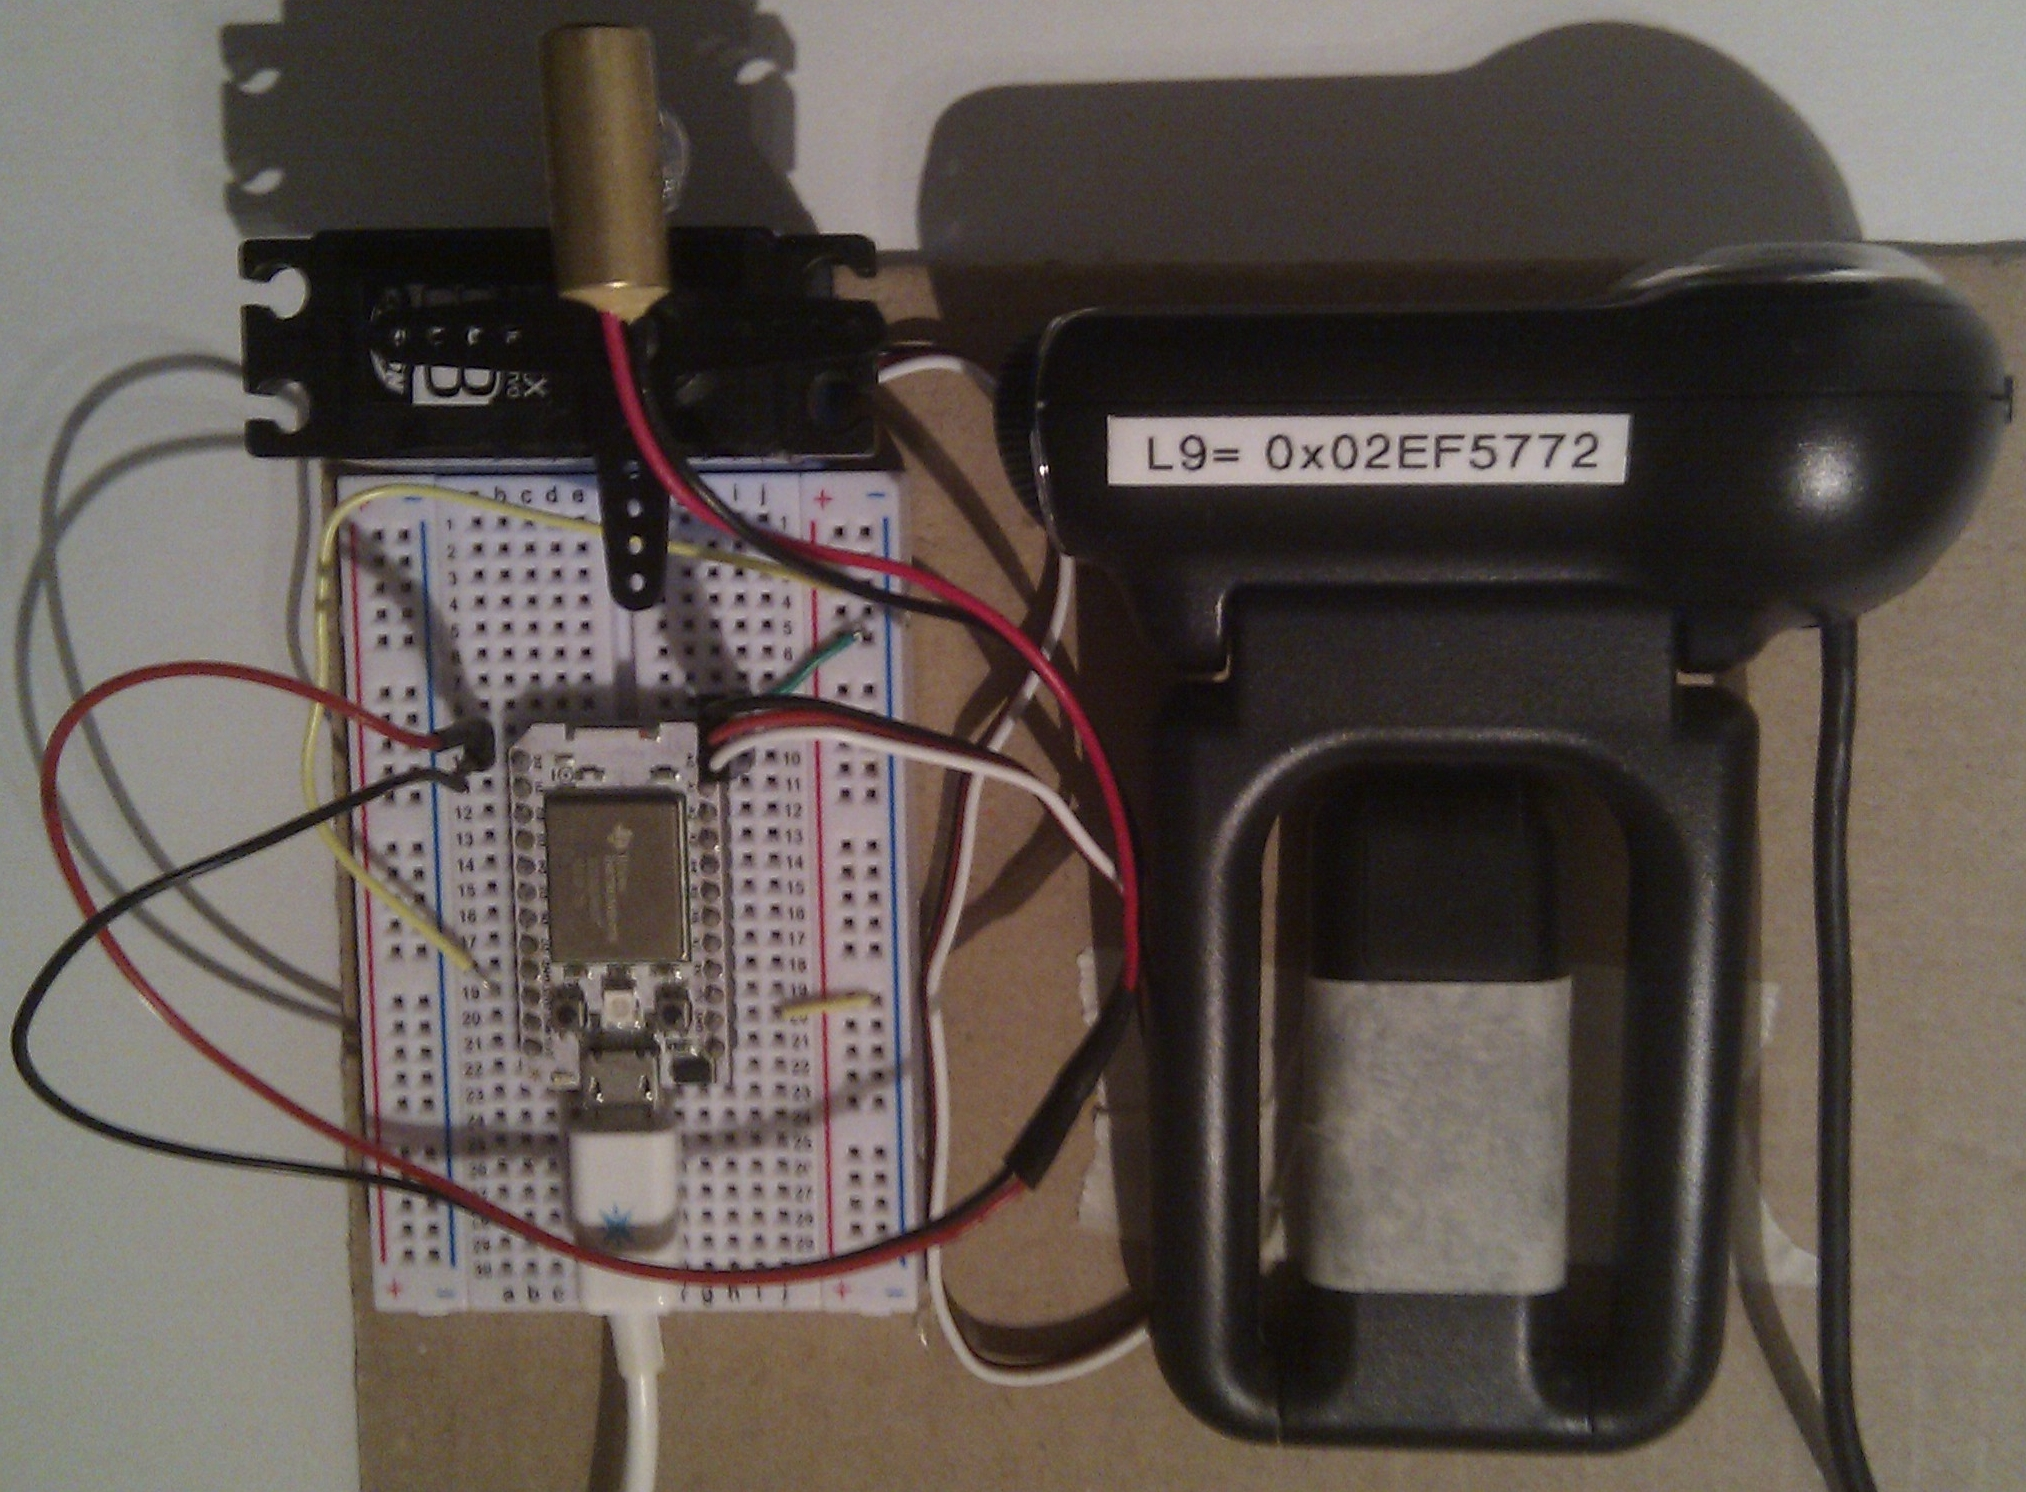
\includegraphics[width=0.8\linewidth]{includes/hardware.jpg}
		\caption{Unsere Hardware}
		\label{fig:hardware}
	\end{figure}

\end{frame}


%\subsection{Linienerkennung}
\begin{frame}
	\frametitlesec
	\framesubtitles{Linienerkennung}

	\textbf{Variante 1 (diff)}\\
	Einfache Linienerkennung durch Differenzbildung:
	\vfill
	\begin{columns}
		\visible<1-4>{\column{.32\linewidth}{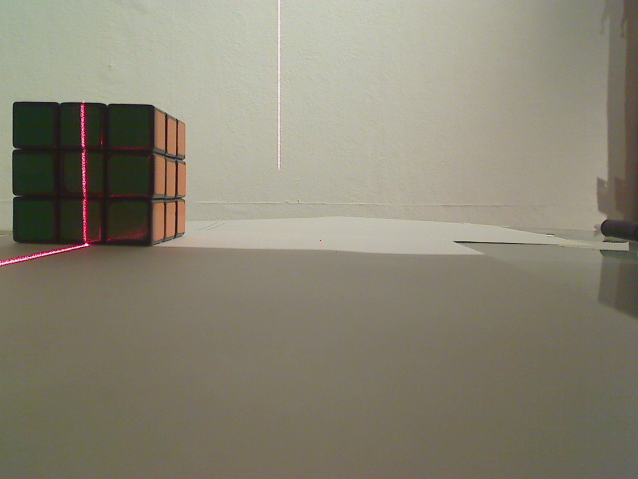
\includegraphics[width=\linewidth]{includes/line_line}}}
		\visible<2-4>{\column{.02\linewidth}{$-$}}
		\visible<2-4>{\column{.32\linewidth}{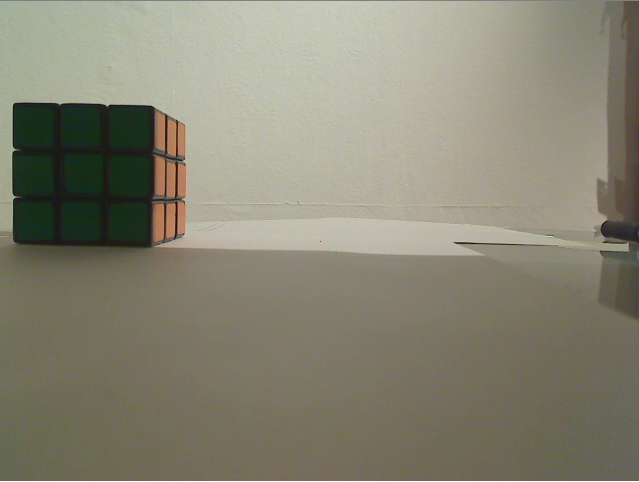
\includegraphics[width=\linewidth]{includes/line_ref}}}
		\visible<3-4>{\column{.02\linewidth}{$=$}}
		\visible<3-4>{\column{.32\linewidth}{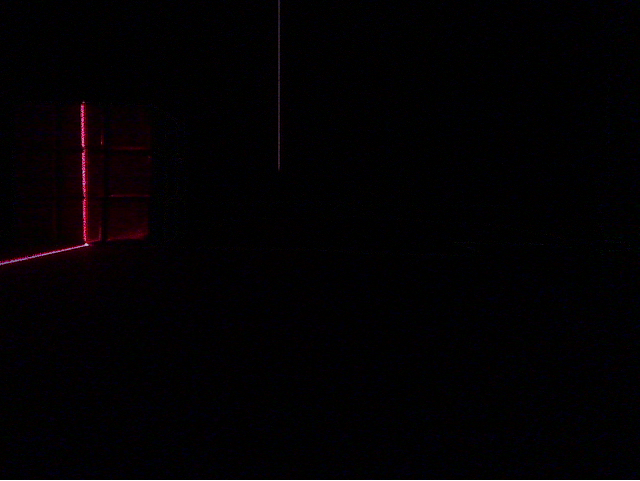
\includegraphics[width=\linewidth]{includes/line_diff}}}
	\end{columns}
	\vfill
	\begin{columns}
%		\column{.02\linewidth}{$\Rightarrow$}
		\visible<4>{\column{.41\linewidth}{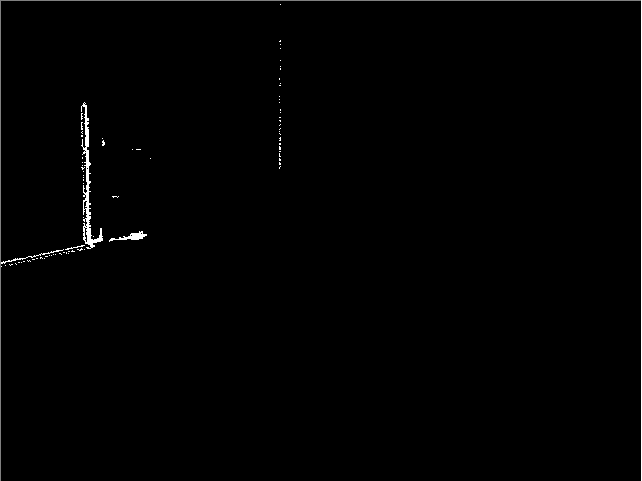
\includegraphics[width=\linewidth]{includes/line_diff_filtered}}}
	\end{columns}

\end{frame}


\begin{frame}
	\frametitlesec
	\framesubtitles{Linienerkennung}

	\textbf{Variante 2 (free)}\\
	Linienerkennung durch kanalweise Mittelwertbildung und logische Verknüpfung:
	\vfill
	\begin{columns}
		\visible<1-2>{\column{.45\linewidth}{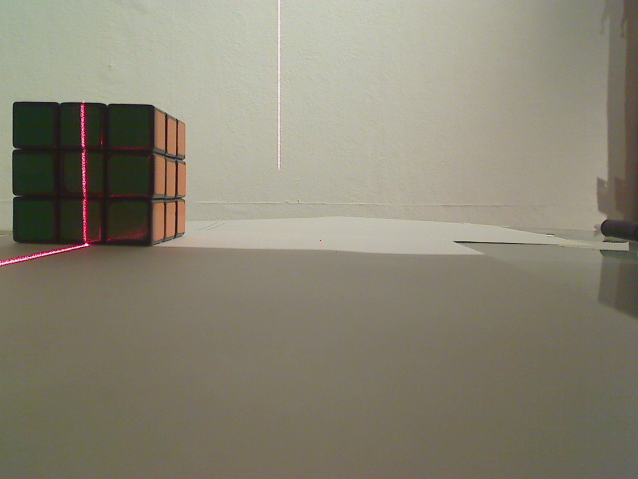
\includegraphics[width=\linewidth]{includes/line_line}}}
		\visible<2>{\column{.05\linewidth}{$\Rightarrow$}}
		\visible<2>{\column{.45\linewidth}{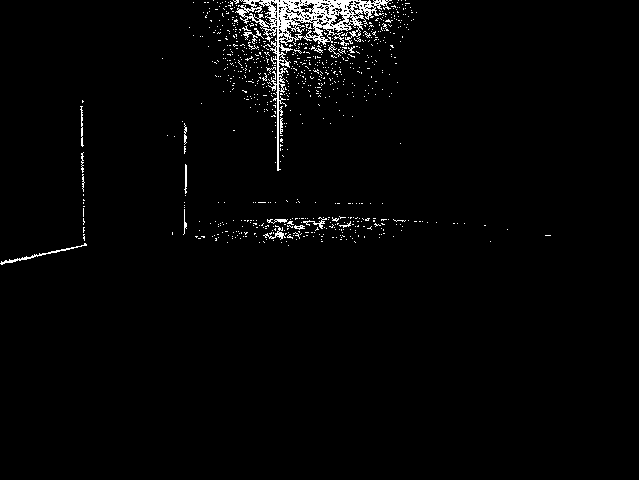
\includegraphics[width=\linewidth]{includes/line_free}}}
	\end{columns}

\end{frame}


%\subsection{Rekonstruktion}
\begin{frame}
	\frametitlesec
	\framesubtitles{Rekonstruktion}

	\begin{columns}
		\small
		\begin{column}{.61\linewidth}
			\begin{itemize}
				\item \textbf{Eingabe:} Normalisierte Bildkoordinaten $(u,v)$ eines Punktes der Laserlinie
				\item \textbf{Schritt 1:} Bestimme $\alpha$, $\beta$, $c$ und $f$
				\item \textbf{Schritt 2:} Berechne $h$:
				\[h = \frac{c \cdot \sin(\alpha) \cdot \sin(\beta)}{\sin(180^\circ - \beta - \alpha)}\]
				\item \textbf{Schritt 3:} Bestimme Koordinaten innerhalb der Szene:
				\[\begin{pmatrix}x\\y\\z\end{pmatrix} = \frac{h}{f} \cdot
				\begin{pmatrix}u\\v\\-f\end{pmatrix}\]
			\end{itemize}
		\end{column}
		\begin{column}{.39\linewidth}
			\hfill\fbox{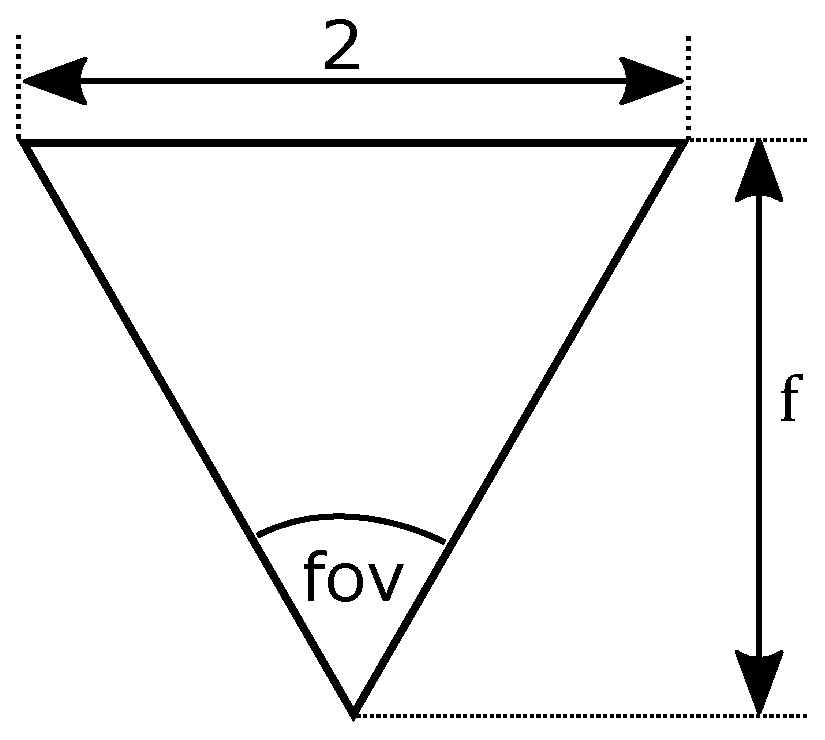
\includegraphics[width=0.9\linewidth]{includes/reconstruction2}}
			\vfill\vspace{3ex}\vfill
			\hfill\fbox{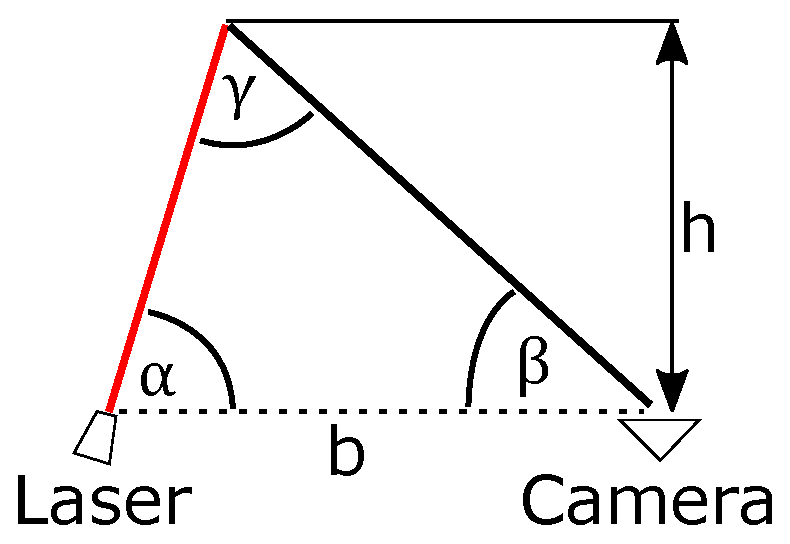
\includegraphics[width=0.9\linewidth]{includes/reconstruction1}}
		\end{column}
	\end{columns}

\end{frame}


%\subsection{Beispiel}
\begin{frame}
	\frametitlesec
	\framesubtitles{Beispiel}

	\begin{overlayarea}{\textwidth}{\textheight}
		\only<1>{
			\begin{figure}
				\centering
				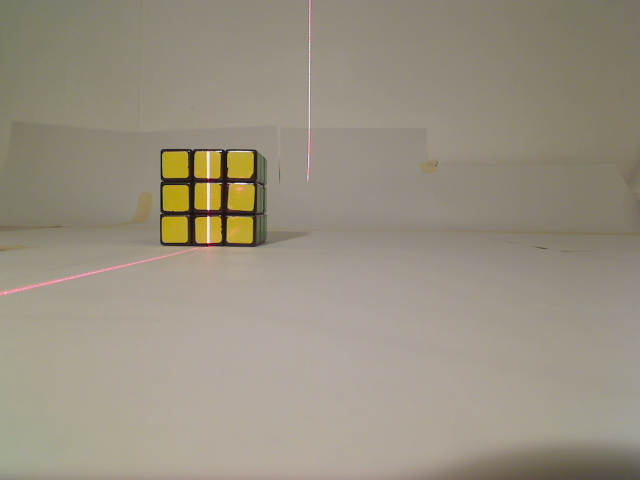
\includegraphics[width=0.8\linewidth]{includes/cap.png}
				\caption{Ausgangsbild}
				\label{fig:example1}
			\end{figure}
		}
		\only<2>{
			\begin{figure}
				\centering
				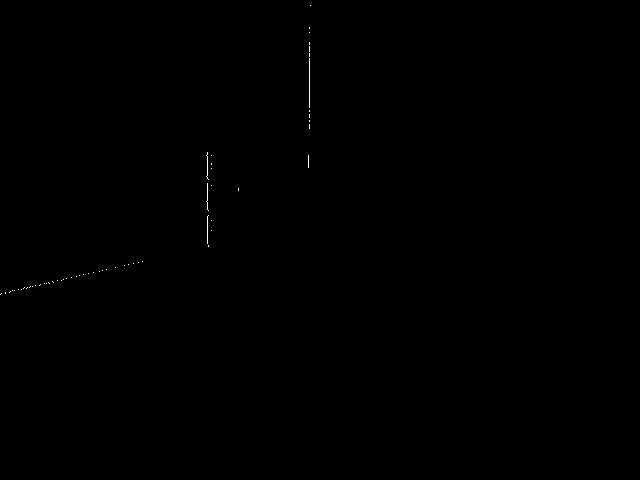
\includegraphics[width=0.8\linewidth]{includes/line.png}
				\caption{Erkannte Linie aus dem Ausgangsbild}
				\label{fig:example2}
			\end{figure}
		}
		\only<3>{
			\begin{figure}
				\centering
				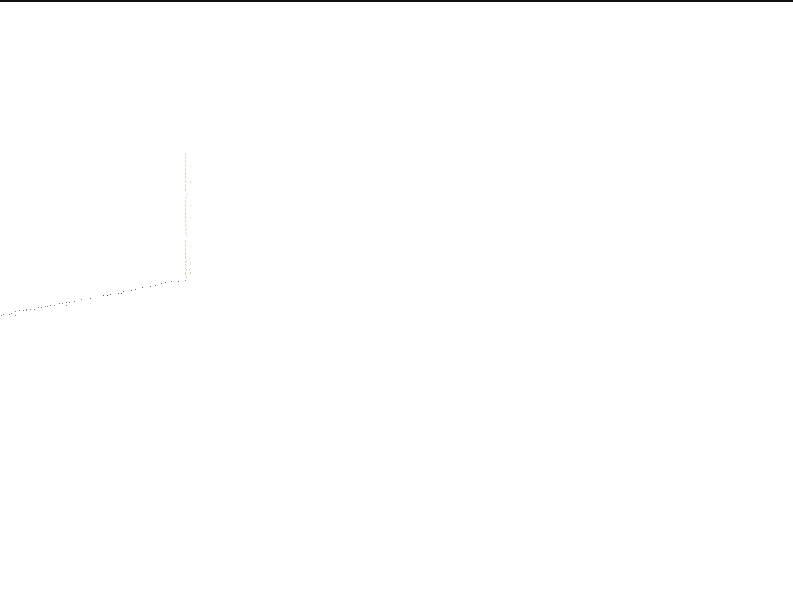
\includegraphics[width=0.8\linewidth]{includes/3d.png}
				\caption{Rekonstruierte Punkte aus der Perspektive der Kamera}
				\label{fig:example3}
			\end{figure}
		}
		\only<4>{
			\begin{figure}
				\centering
				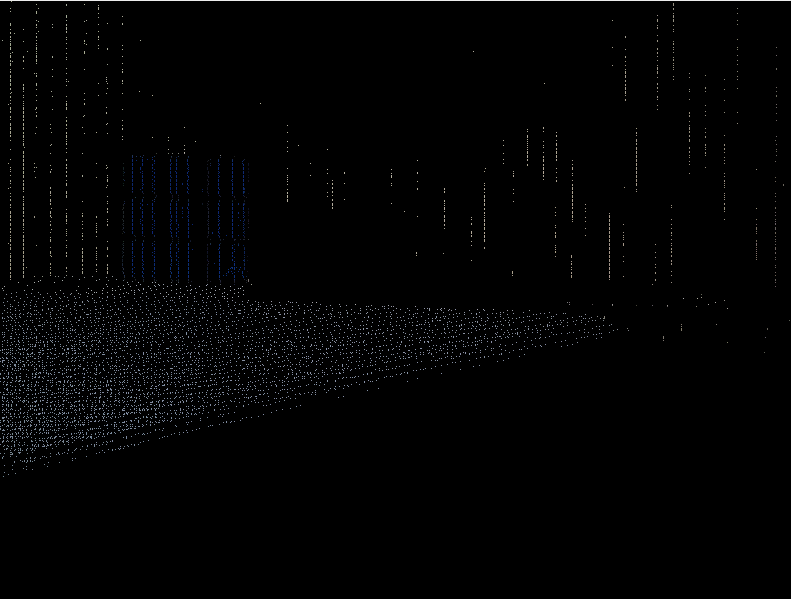
\includegraphics[width=0.8\linewidth]{includes/3d_2.png}
				\caption{Rekonstruierte Punkte der Szene (1)}
				\label{fig:example4}
			\end{figure}
		}
		\only<5>{
			\begin{figure}
				\centering
				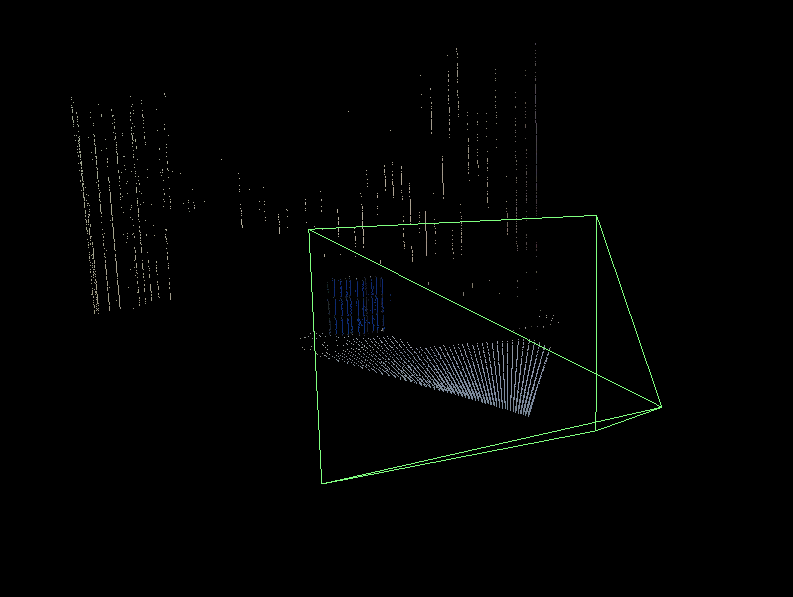
\includegraphics[width=0.8\linewidth]{includes/3d_3.png}
				\caption{Rekonstruierte Punkte der Szene (2)}
				\label{fig:example5}
			\end{figure}
		}
		\only<6>{
			\begin{figure}
				\centering
				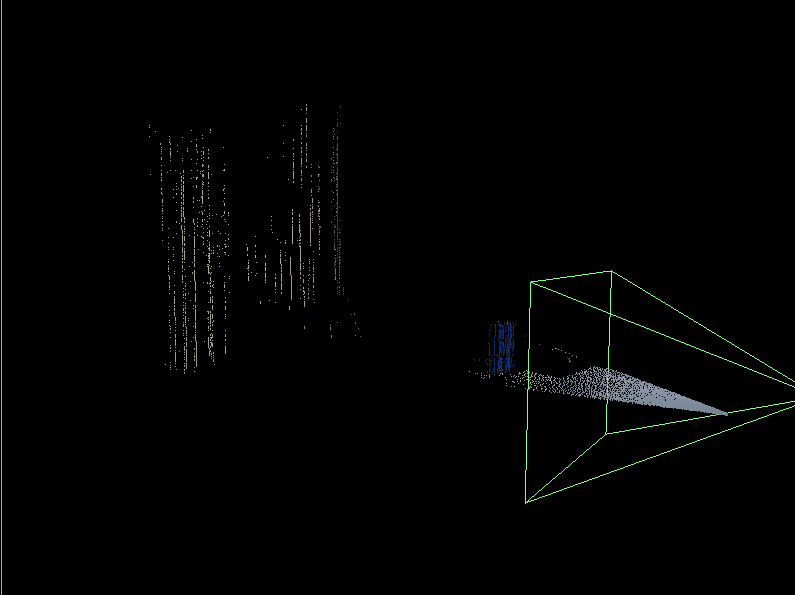
\includegraphics[width=0.8\linewidth]{includes/3d_4.png}
				\caption{Rekonstruierte Punkte der Szene (3)}
				\label{fig:example6}
			\end{figure}
		}
	\end{overlayarea}

\end{frame}

% ---------------------------------------------------------------------------- %

\section{Probleme}
%\subsection{Organisatorisches}
\begin{frame}
	\frametitlesec

	\begin{itemize}
		\item Viel Zeit bei der Planung verloren
		\begin{itemize}
			\item Fehlende Erfahrung bei der Strukturierung solcher Anwendungen
			\item Uneinigkeit bei Schwerpunkten und Verfahren
		\end{itemize}
		\vfill
		\item Montage des Setups
		\vfill
		\item Hardware als Ursache für Ungenauigkeiten
		\begin{itemize}
			\item Kleine Fehler bei der Montage
			\item Vermessung des Setups problematisch
		\end{itemize}
		\vfill
		\item Linienerkennung
		\begin{itemize}
			\item Hintergrundfarbe
			\item Beleuchtung
		\end{itemize}
	\end{itemize}

\end{frame}


\begin{frame}
	\frametitlesec

	\begin{figure}
		\centering
		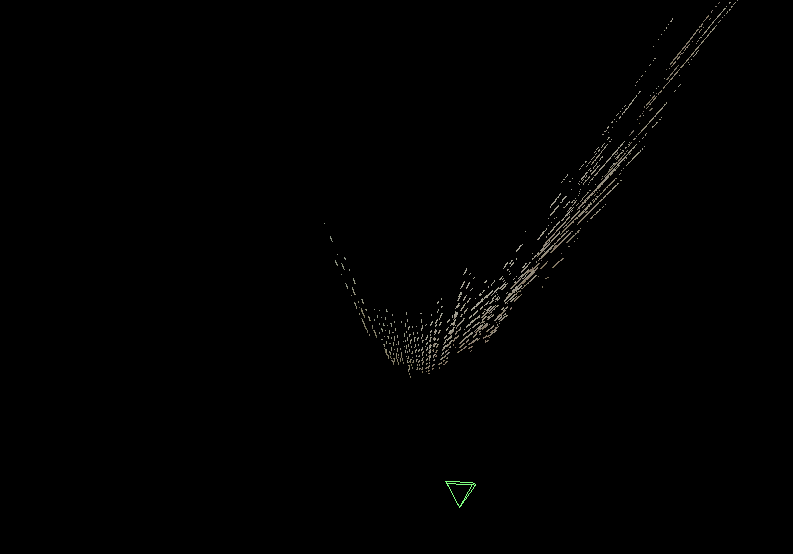
\includegraphics[width=0.85\linewidth]{includes/krumm.png}
		\caption{Scan einer geraden Wand bei falscher Kalibrierung}
		\label{fig:hw_calibration_fault}
	\end{figure}

\end{frame}

% ---------------------------------------------------------------------------- %

\section{Ergebnisse}

\begin{frame}
	\frametitlesec
%	\framesubtitles{Messungen}

	\textbf{Messungen}

	\begin{figure}
		\begin{minipage}{0.32\linewidth}
			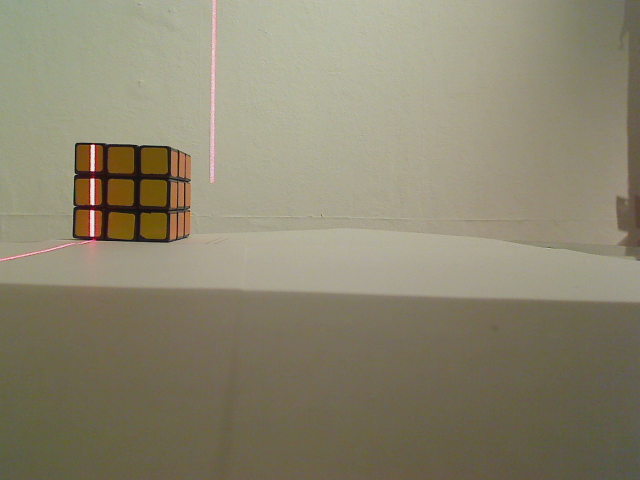
\includegraphics[width=\linewidth]{includes/test_repeat_1}
		\end{minipage}
		\hfill
		\begin{minipage}{0.32\linewidth}
			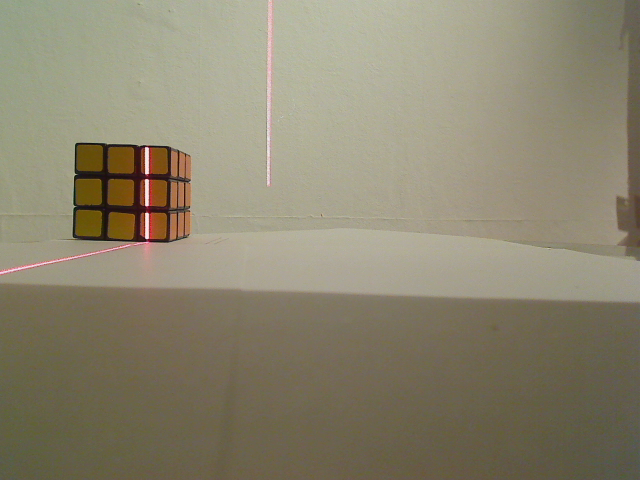
\includegraphics[width=\linewidth]{includes/test_repeat_2}
		\end{minipage}
		\hfill
		\begin{minipage}{0.32\linewidth}
			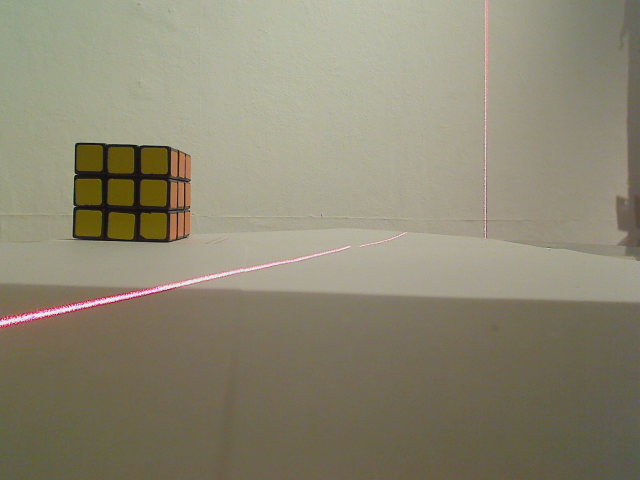
\includegraphics[width=\linewidth]{includes/test_repeat_3}
		\end{minipage}
	\end{figure}

	\begin{itemize}
		\item Abtastung eines Zauberwürfels (Rubik's Cube)
		\item Messungen mit unterschiedlicher Zielsetzung
		\begin{itemize}
			\item Wiederholte Messungen
			\item Variation der Entfernungen
			\item Variation der Farben
			\item Variation der Beleuchtung
		\end{itemize}
	\end{itemize}

\end{frame}


\begin{frame}
	\frametitlesec
%	\framesubtitles{Auffälligkeiten}

	\textbf{Auffälligkeiten}

	\begin{figure}
		\begin{minipage}{0.32\linewidth}
			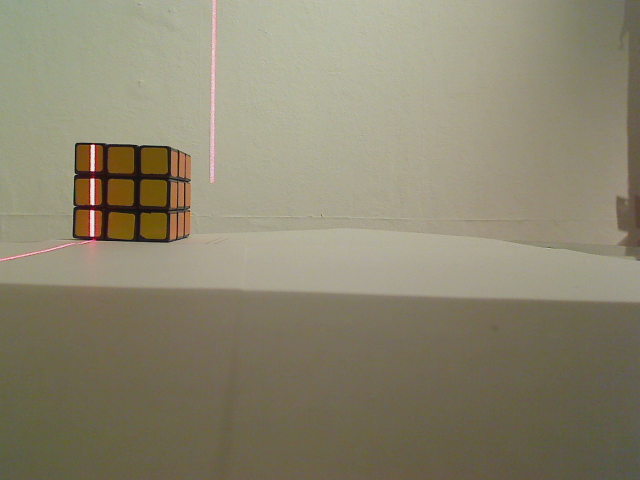
\includegraphics[width=\linewidth]{includes/test_repeat_1}
		\end{minipage}
		\hfill
		\begin{minipage}{0.32\linewidth}
			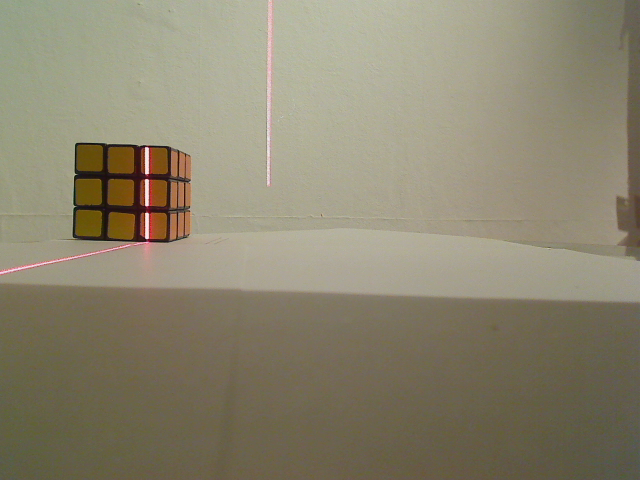
\includegraphics[width=\linewidth]{includes/test_repeat_2}
		\end{minipage}
		\hfill
		\begin{minipage}{0.32\linewidth}
			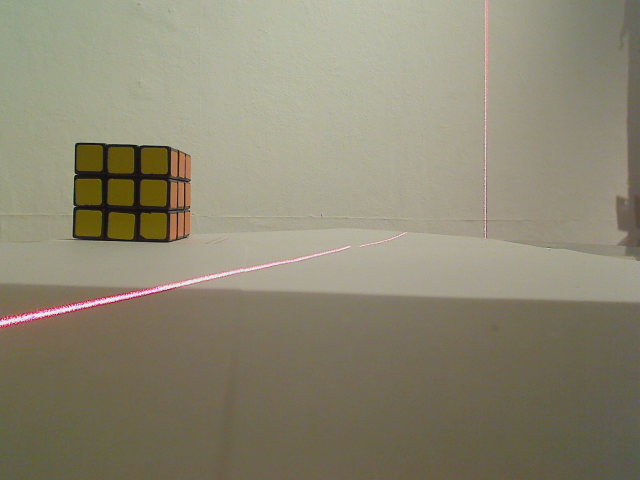
\includegraphics[width=\linewidth]{includes/test_repeat_3}
		\end{minipage}
	\end{figure}

	\begin{itemize}
		\item 12\% bis 17\% größere Entfernung
		\begin{itemize}
			\item 300~mm $\rightarrow$ 338~mm - 341~mm
		\end{itemize}
		\item Schwache Beleuchtung beeinträchtigt die Ergebnisse
		\begin{itemize}
			\item Standartabweichung (diff): 15~mm $\rightarrow$ 98~mm
		\end{itemize}
		\item Ergebnis stark von Linienerkennung beeinflusst
	\end{itemize}

\end{frame}

% ---------------------------------------------------------------------------- %

\section{Zusammenfassung}
\begin{frame}
	\frametitlesec

	\begin{columns}
	\column<1->{.45\linewidth}{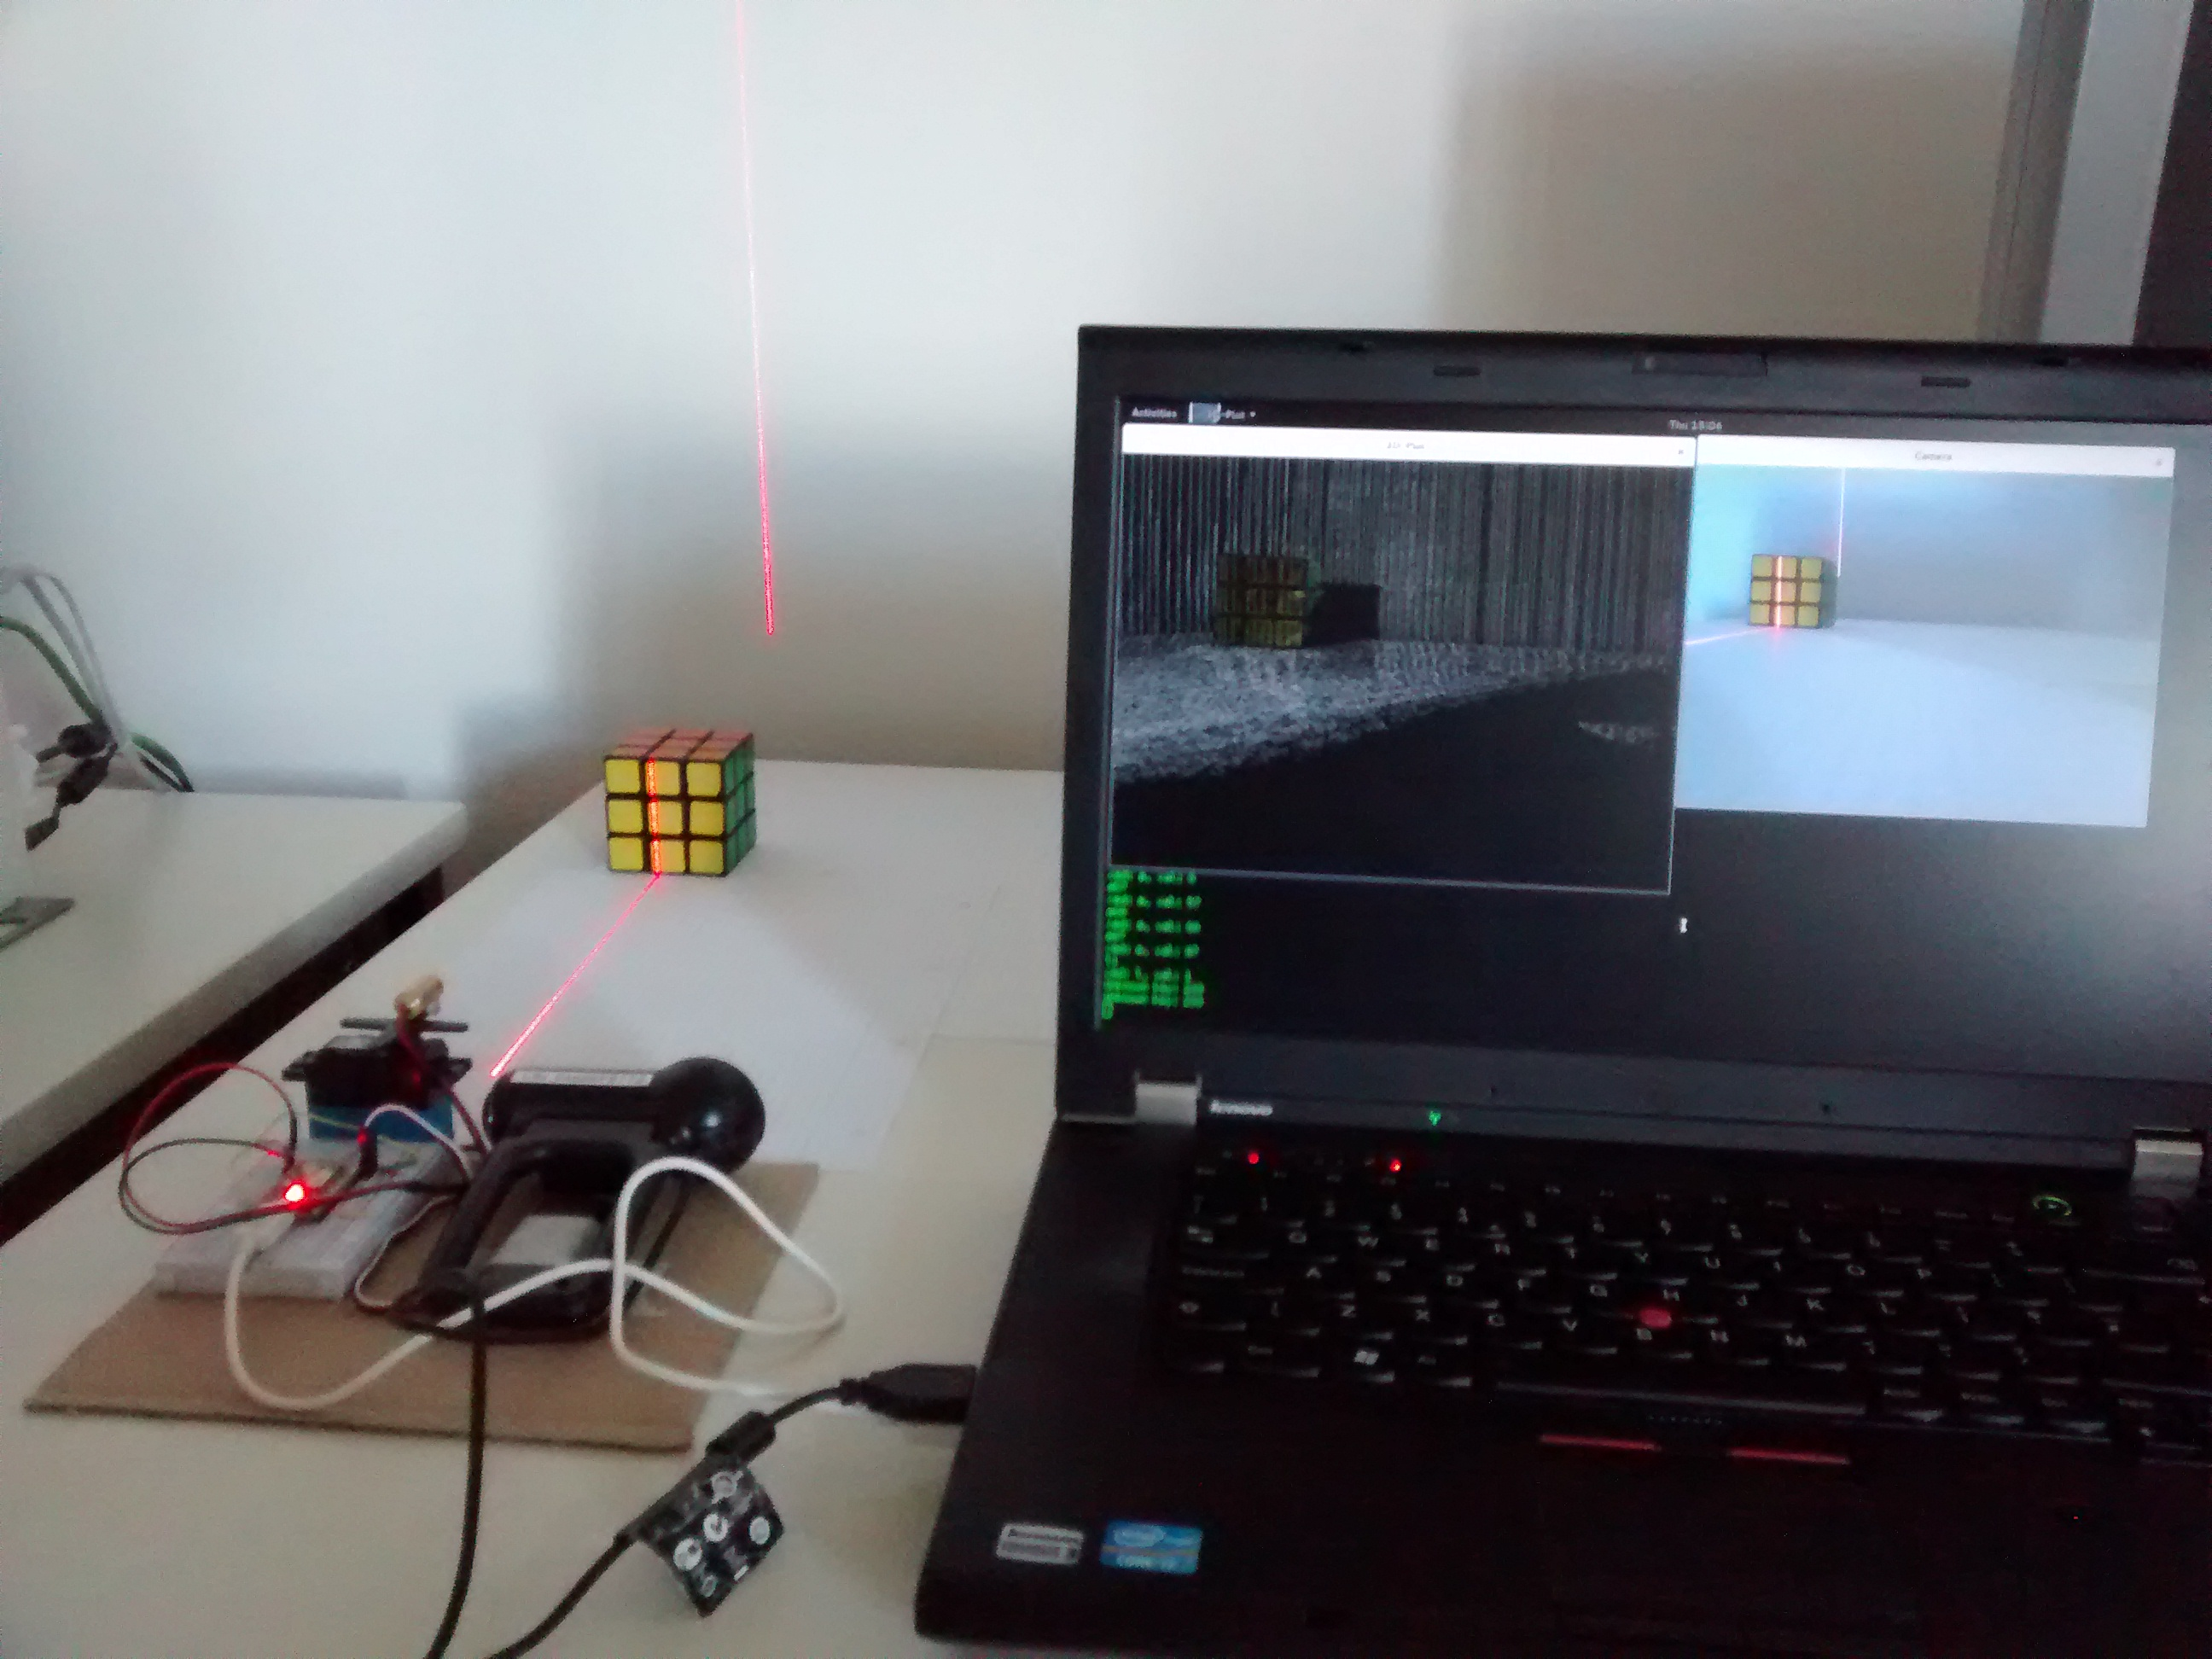
\includegraphics[width=\linewidth]{includes/setup}}
	\column<2->{.45\linewidth}{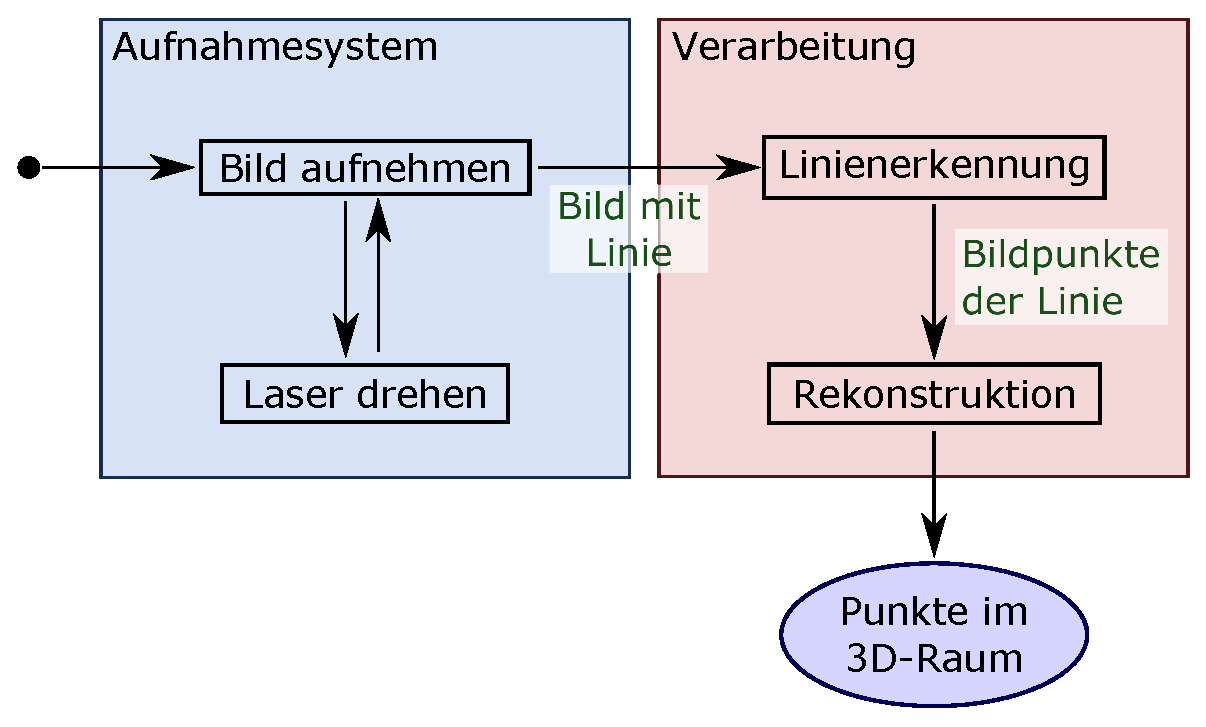
\includegraphics[width=\linewidth]{includes/blockbild}}
	\end{columns}
	\begin{columns}
	\column{.45\linewidth}{}
	\column<3->{.45\linewidth}{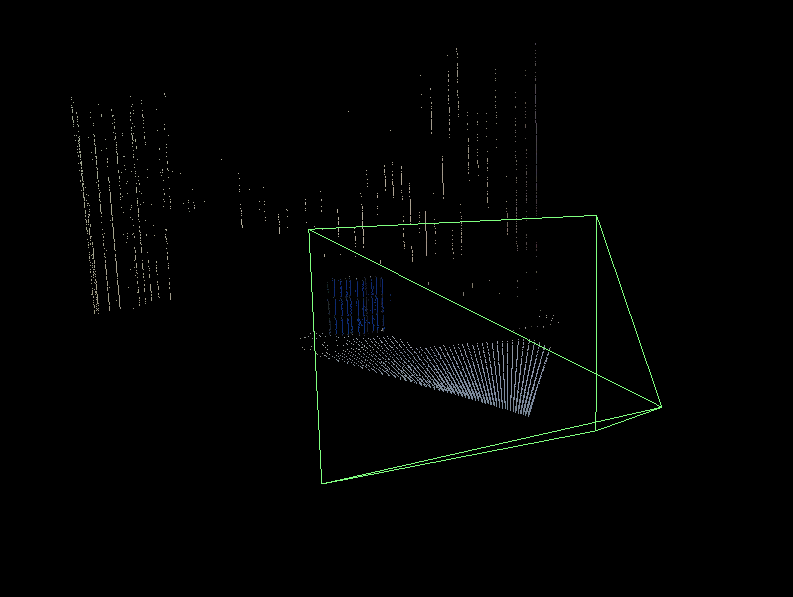
\includegraphics[width=\linewidth]{includes/3d_3.png}}
	\end{columns}

\end{frame}

% ---------------------------------------------------------------------------- %

\begin{frame}
	\frametitle{\mbox{}}
	\center \LARGE Vielen Dank für eure Aufmerksamkeit!
\end{frame}

% ---------------------------------------------------------------------------- %

\end{document}
